\documentclass{standalone}
\usepackage{tikz}
\usetikzlibrary{positioning,arrows.meta,calc}
\usepackage{amsmath}
\usepackage{listofitems}
\usepackage[outline]{contour}
\contourlength{1.4pt}
\usetikzlibrary{fit,positioning}

% COLORS
\usepackage{xcolor}
\colorlet{myred}{red!80!black}
\colorlet{myblue}{blue!80!black}
\colorlet{mybluee}{myblue!80!black}
\colorlet{mygreen}{green!60!black}
\colorlet{myorange}{orange!70!red!60!black}
\colorlet{mydarkred}{red!30!black}
\colorlet{mydarkblue}{blue!40!black}
\colorlet{mydarkgreen}{green!30!black}

\begin{document}

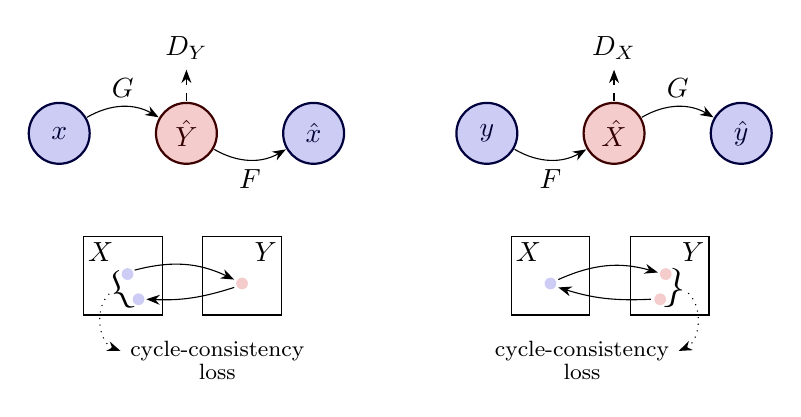
\begin{tikzpicture}[
    >=Stealth, % for default LaTeX arrow head
    box/.style={thick,circle,minimum size=22,inner sep=0.5,outer sep=0.6},
    bigbox/.style={draw, minimum width=10mm, minimum height=10mm}
]

% Upper diagram
\node[blue!20!black,draw=myblue!30!black,fill=myblue!20, box] (x) {$x$};
\node[red!20!black,draw=myred!30!black,fill=myred!20, box, right=8mm of x] (Y) {$\hat{Y}$};
\node[blue!20!black,draw=myblue!30!black,fill=myblue!20, box, right=8mm of Y] (xhat) {$\hat{x}$};

\node[blue!20!black,draw=myblue!30!black,fill=myblue!20, box, right=30mm of Y] (y) {$y$};
\node[red!20!black,draw=myred!30!black,fill=myred!20, box, right=8mm of y] (X) {$\hat{X}$};
\node[blue!20!black,draw=myblue!30!black,fill=myblue!20, box, right=8mm of X] (yhat) {$\hat{y}$};

\draw[->] (x) to[bend left=30] node[above] {$G$} (Y);
\draw[->] (Y) to[bend right=30] node[below] {$F$} (xhat);

\draw[->] (y) to[bend right=30] node[below] {$F$} (X);
\draw[->] (X) to[bend left=30] node[above] {$G$} (yhat);

% Vertical arrow
\draw[->, dashed] (Y.north) -- +(0,4mm) node[above] {$D_Y$};
\draw[->, dashed] (X.north) -- +(0,4mm) node[above] {$D_X$};

% Lower diagram
\node[bigbox, yshift=0.2cm, below=15mm of $(x)!0.5!(Y)$, label={[xshift=-0.28cm, yshift=-0.45cm]$X$}] (X2) {};
\node[bigbox, right=5mm of X2, label={[xshift=0.3cm, yshift=-0.45cm]$Y$}] (Y2) {};

% Dots in lower boxes
\node[circle, fill=myblue!20, inner sep=1.5pt] at ($(X2.center)+(0.6mm,0.2mm)$) {};
\node[circle, fill=myblue!20, inner sep=1.5pt] at ($(X2.center)+(2mm,-3mm)$) {};
\node[circle, fill=myred!20, inner sep=1.5pt] at ($(Y2.center)+(0,-1mm)$) {};

% Arrows in lower diagram
\draw[->] ($(X2.center)+(1.5mm,0.7mm)$) to[bend left=20] ($(Y2.center)+(-1mm,-0.5mm)$);
\draw[->] ($(Y2.center)+(-1mm,-1.5mm)$) to[bend left=10] ($(X2.center)+(3mm,-3mm)$);

% Cycle-consistency loss text and dotted line
\node[inner sep=1.5pt, rotate=23] at ($(X2.center)+(-0.3mm,-2mm)$) {\Large \{};
\node[below=2mm of X2, xshift=1.2cm] (cycle) {\footnotesize cycle-consistency};
\node[below=-2mm of cycle] (loss) {\footnotesize loss};
\draw[dotted, <-] (cycle.west) to[bend left=60] ($(X2.center)+(-1.5mm,-2.1mm)$);

\node[bigbox, yshift=0.2cm, below=15mm of $(y)!0.5!(X)$, label={[xshift=-0.28cm, yshift=-0.45cm]$X$}] (X) {};
\node[bigbox, right=5mm of X, label={[xshift=0.3cm, yshift=-0.45cm]$Y$}] (Y2) {};

% Dots in lower boxes
\node[circle, fill=myred!20, inner sep=1.5pt] at ($(Y2.center)+(-0.5mm,0.2mm)$) {};
\node[circle, fill=myred!20, inner sep=1.5pt] at ($(Y2.center)+(-1.2mm,-3mm)$) {};
\node[circle, fill=myblue!20, inner sep=1.5pt] at ($(X.center)+(0,-1mm)$) {};

% Arrows in lower diagram
\draw[->] ($(X.center)+(1mm,-0.5mm)$) to[bend left=20] ($(Y2.center)+(-1.5mm,0.4mm)$);
\draw[->] ($(Y2.center)+(-2.4mm,-3mm)$) to[bend left=10] ($(X.center)+(1mm,-1.5mm)$);

% Cycle-consistency loss text and dotted line
\node[inner sep=1.5pt, rotate=168] at ($(Y2.center)+(0.8mm,-1.7mm)$) {\Large \{};
\node[below=2mm of X, xshift=0.4cm] (cycle) {\footnotesize cycle-consistency};
\node[below=-2mm of cycle] (loss) {\footnotesize loss};
\draw[dotted, <-] (cycle.east) to[bend right=60] ($(Y2.center)+(2mm,-1.9mm)$);

\end{tikzpicture}
\end{document}